\begin{frame}{Salvemos a ED usando RoR}
  ¿Qué es Ruby on Rails?
  \begin{tabular}{l c}
    \parbox{0.5\textwidth}{
      \begin{itemize}
        \item Framework de desarrollo web.
        \item Basado en Ruby.
        \item M.V.C.
        \item CoC
        \item Incluye todos los procesos del desarrollo web.
        \item Apoyado por gemas.
      \end{itemize}
    } &
    \raisebox{-0.5\totalheight}{
\includegraphics[scale=0.2]{img/ror}}
  \end{tabular}
\end{frame}

\begin{frame}{El modelo M.V.C. de RoR}
  \centering
  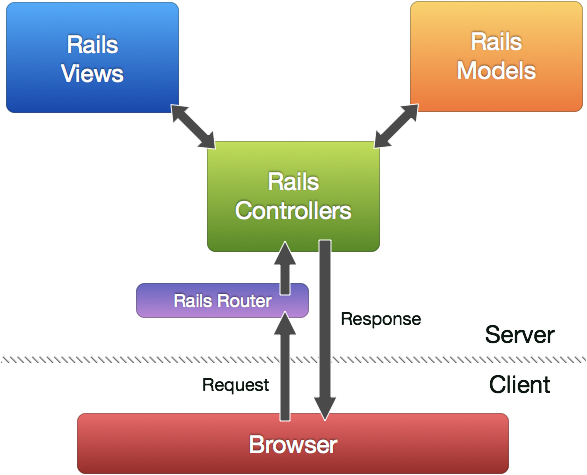
\includegraphics[scale=0.3]{img/railsmvc}
\end{frame}

\begin{frame}[fragile]{Convenciones sobre la configuración}
  Lo básico:

  \pause

  \begin{tabular}{l l}
    \parbox{0.5\textwidth}{
      app/models/:
      \begin{itemize}
        \item ActiveRecord::Base.
        \item Clases $\leftrightarrow$ Tablas.
        \item Infinidad de métodos predefinidos.
      \end{itemize}
    } \pause &
    \begin{lstlisting}
# app/models/user.rb
class User < ActiveRecord::Base
  belongs_to :company # modelo Company
  has_many :associates # modelo Associate
  has_one :session # modelo Sessions

  ...
end
    \end{lstlisting} \pause \\

    \parbox{0.5\textwidth}{
      app/controllers/:
      \begin{itemize}
        \item ActionController::Base.
        \item Manejan la lógica.
        \item Reciben peticiones.
      \end{itemize}
    } \pause &
    \begin{lstlisting}
# app/controllers/users_controller.rb
class UsersController < ActionController::Base
  def index
    @users = User.where( ... )
  end

  ...
end
    \end{lstlisting} \pause \\

    \parbox{0.5\textwidth}{
      app/views:
      \begin{itemize}
        \item Archivos .erb.
        \item Contienen las interfaces.
        \item HTML, Haml.
      \end{itemize}
    } \pause &
    \begin{lstlisting}[language=HTML]
<!-- app/views/users/index.html.erb -->
...
<% @users.each do |user| % >
  <p> <% = user.name % > </p>
<% end % >
...
    \end{lstlisting}
  \end{tabular}
\end{frame}

\begin{frame}{Apoyo de las gemas (demos)}
  \begin{tabular}{l l}
    \raisebox{-0.5\totalheight}{
\includegraphics[scale=0.4]{img/rails_gems}} &
    \pause 

    \parbox{0.5\textwidth}{
      \begin{itemize}
        \item Squeel $\rightarrow$ Mejor SQL. \pause
        \item Pry $\rightarrow$ Depuración. \pause
        \item CanCan $\rightarrow$ Autorización. \pause
        \item Authlogic $\rightarrow$ Autenticación. \pause
        \item simple\_form, prawn, nested\_form, spreadsheet, haml, zeus,
        jquery\_rails...
      \end{itemize}
    }
  \end{tabular}

  \begin{center}
    \textbf{INVIERTE TU TIEMPO EN TU PROYECTO}
  \end{center}
\end{frame}
